\documentclass[11pt]{article}

\usepackage[margin=0.82in,headheight=15pt,footskip=30pt]{geometry}
\usepackage{fontspec}
\setmainfont{DejaVu Serif}
\setsansfont{DejaVu Sans}
\setmonofont{DejaVu Sans Mono}[Scale=0.82]
\usepackage{microtype}
\usepackage{amsmath,amssymb,mathtools}
\usepackage{amsthm}
\usepackage{booktabs,longtable,array,tabularx}
\usepackage{graphicx}
\usepackage{float}
\usepackage{caption}
\usepackage{enumitem}
\usepackage{xcolor}
\usepackage{tikz}
\usetikzlibrary{arrows.meta,positioning,calc,fit,shapes.geometric,decorations.pathreplacing}
\usepackage{pgfplots}
\pgfplotsset{compat=1.18}
\usepackage[most]{tcolorbox}
\usepackage{listings}
\usepackage{upquote}
\usepackage{xurl}
\usepackage{hyperref}
\usepackage{bookmark}
\usepackage{fancyhdr}
\usepackage{lastpage}
\usepackage{titlesec}
\usepackage{needspace}
\usepackage{etoolbox}
\usepackage{setspace}
\usepackage{tocloft}

\definecolor{HilbertBlue}{HTML}{245B8A}
\definecolor{HilbertTeal}{HTML}{2E7D73}
\definecolor{HilbertGold}{HTML}{A56B16}
\definecolor{HilbertRed}{HTML}{9A3B3B}
\definecolor{HilbertPurple}{HTML}{66508C}
\definecolor{HilbertGray}{HTML}{4F5B66}
\definecolor{SoftBlue}{HTML}{EAF1F8}
\definecolor{SoftTeal}{HTML}{E8F4F1}
\definecolor{SoftGold}{HTML}{FAF2E3}
\definecolor{SoftRed}{HTML}{F8EAEA}
\definecolor{SoftPurple}{HTML}{EFEAF7}
\definecolor{SoftGray}{HTML}{EEF0F2}

\hypersetup{
  colorlinks=true,
  linkcolor=HilbertBlue,
  urlcolor=HilbertBlue,
  citecolor=HilbertTeal,
  pdftitle={Hilbert Space Filling Curve-Style Theorem Search v0.5.3},
  pdfauthor={Brian Tenneson}
}

\setcounter{secnumdepth}{2}
\setcounter{tocdepth}{2}
\setlength{\cftsecnumwidth}{2.9em}
\setlength{\cftsubsecindent}{2.0em}
\setlength{\cftsubsecnumwidth}{3.7em}
\renewcommand{\cftsecleader}{\cftdotfill{\cftdotsep}}
\renewcommand{\cftsecpagefont}{\bfseries\sffamily\color{HilbertBlue}}
\renewcommand{\cfttoctitlefont}{\Large\bfseries\sffamily\color{HilbertBlue}}
\setlength{\cftbeforetoctitleskip}{0pt}
\setlength{\cftaftertoctitleskip}{0.7em}
\setlength{\parindent}{0pt}
\setlength{\parskip}{0.55em}
\setlength{\emergencystretch}{3em}
\setlist[itemize]{topsep=0.35em,itemsep=0.25em,leftmargin=1.55em}
\renewcommand{\arraystretch}{1.15}
\newcommand{\real}[1]{#1}
\providecommand{\tightlist}{\setlength{\itemsep}{0pt}\setlength{\parskip}{0pt}}

\titleformat{\section}{\Large\bfseries\sffamily\color{HilbertBlue}}{\thesection}{0.75em}{}[\color{HilbertBlue!45}\titlerule]
\titleformat{\subsection}{\large\bfseries\sffamily\color{HilbertTeal}}{\thesubsection}{0.65em}{}
\titleformat{\subsubsection}{\normalsize\bfseries\sffamily\color{HilbertGray}}{\thesubsubsection}{0.6em}{}

\pagestyle{fancy}
\fancyhf{}
\fancyhead[L]{\small\sffamily Hilbert Space Filling Curve-Style Theorem Search}
\fancyhead[R]{\small\sffamily v0.5.3}
\fancyfoot[L]{\small\sffamily Brian Tenneson}
\fancyfoot[R]{\small\sffamily Page \thepage\ of \pageref*{LastPage}}
\renewcommand{\headrulewidth}{0.35pt}
\renewcommand{\footrulewidth}{0.25pt}
\fancypagestyle{plain}{%
  \fancyhf{}%
  \fancyhead[L]{\small\sffamily Hilbert Space Filling Curve-Style Theorem Search}%
  \fancyhead[R]{\small\sffamily v0.5.3}%
  \fancyfoot[L]{\small\sffamily Brian Tenneson}%
  \fancyfoot[R]{\small\sffamily Page \thepage\ of \pageref*{LastPage}}%
  \renewcommand{\headrulewidth}{0.35pt}%
  \renewcommand{\footrulewidth}{0.25pt}%
}

\lstdefinestyle{hilbertcode}{
  language=Python,
  basicstyle=\ttfamily\scriptsize,
  numbers=left,
  numberstyle=\tiny\color{HilbertGray},
  numbersep=8pt,
  frame=single,
  rulecolor=\color{HilbertGray!35},
  backgroundcolor=\color{SoftGray!45},
  breaklines=true,
  breakatwhitespace=false,
  showstringspaces=false,
  tabsize=4,
  columns=fullflexible,
  keepspaces=true,
  captionpos=b,
  xleftmargin=1.8em,
  framexleftmargin=1.2em,
  aboveskip=0.8em,
  belowskip=0.8em
}

\newtheoremstyle{hilberttheorem}% name
  {0.9em}% space above
  {0.9em}% space below
  {\itshape}% body font
  {}% indent
  {\bfseries\sffamily\color{HilbertBlue}}% head font
  {.}% punctuation
  {0.5em}% after head
  {}% head spec
\theoremstyle{hilberttheorem}
\newtheorem{theorem}{Theorem}
\newtheorem{conjecture}{Conjecture}
\newtheorem{proposition}{Proposition}

\AtBeginEnvironment{proof}{\small}

% ---------- LaTeX-native figures ----------
\newcommand{\HistoryJigsawFigure}{%
\begin{figure}[H]
\centering
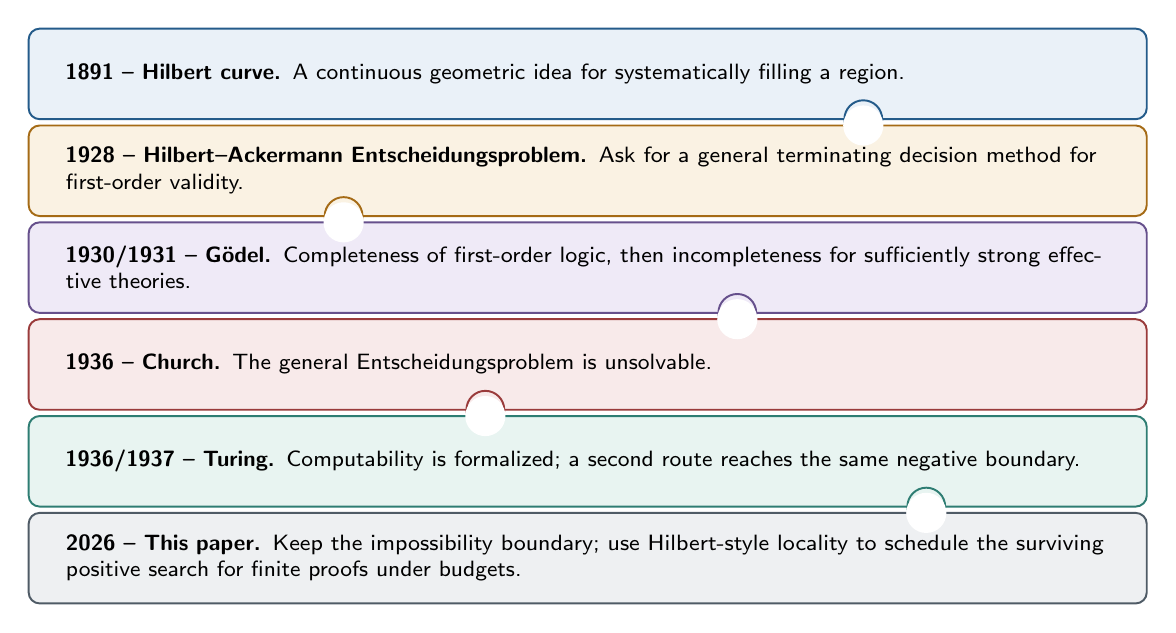
\begin{tikzpicture}[x=1cm,y=1cm,font=\sffamily\footnotesize]
  % Draw manually so colors and text remain independently controllable.
  \filldraw[rounded corners=4pt,fill=SoftBlue,draw=HilbertBlue,line width=.7pt] (0,6.25) rectangle (14.2,7.40);
  \filldraw[fill=SoftBlue,draw=HilbertBlue,line width=.7pt] (10.6,6.25) circle (.24);
  \node[anchor=west,text width=13.25cm] at (.35,6.83) {\textbf{1891 -- Hilbert curve.} A continuous geometric idea for systematically filling a region.};

  \filldraw[rounded corners=4pt,fill=SoftGold,draw=HilbertGold,line width=.7pt] (0,5.02) rectangle (14.2,6.17);
  \fill[white] (10.6,6.17) circle (.255);
  \filldraw[fill=SoftGold,draw=HilbertGold,line width=.7pt] (4.0,5.02) circle (.24);
  \node[anchor=west,text width=13.25cm] at (.35,5.60) {\textbf{1928 -- Hilbert--Ackermann Entscheidungsproblem.} Ask for a general terminating decision method for first-order validity.};

  \filldraw[rounded corners=4pt,fill=SoftPurple,draw=HilbertPurple,line width=.7pt] (0,3.79) rectangle (14.2,4.94);
  \fill[white] (4.0,4.94) circle (.255);
  \filldraw[fill=SoftPurple,draw=HilbertPurple,line width=.7pt] (9.0,3.79) circle (.24);
  \node[anchor=west,text width=13.25cm] at (.35,4.37) {\textbf{1930/1931 -- G\"odel.} Completeness of first-order logic, then incompleteness for sufficiently strong effective theories.};

  \filldraw[rounded corners=4pt,fill=SoftRed,draw=HilbertRed,line width=.7pt] (0,2.56) rectangle (14.2,3.71);
  \fill[white] (9.0,3.71) circle (.255);
  \filldraw[fill=SoftRed,draw=HilbertRed,line width=.7pt] (5.8,2.56) circle (.24);
  \node[anchor=west,text width=13.25cm] at (.35,3.14) {\textbf{1936 -- Church.} The general Entscheidungsproblem is unsolvable.};

  \filldraw[rounded corners=4pt,fill=SoftTeal,draw=HilbertTeal,line width=.7pt] (0,1.33) rectangle (14.2,2.48);
  \fill[white] (5.8,2.48) circle (.255);
  \filldraw[fill=SoftTeal,draw=HilbertTeal,line width=.7pt] (11.4,1.33) circle (.24);
  \node[anchor=west,text width=13.25cm] at (.35,1.91) {\textbf{1936/1937 -- Turing.} Computability is formalized; a second route reaches the same negative boundary.};

  \filldraw[rounded corners=4pt,fill=SoftGray,draw=HilbertGray,line width=.7pt] (0,.10) rectangle (14.2,1.25);
  \fill[white] (11.4,1.25) circle (.255);
  \node[anchor=west,text width=13.25cm] at (.35,.68) {\textbf{2026 -- This paper.} Keep the impossibility boundary; use Hilbert-style locality to schedule the surviving positive search for finite proofs under budgets.};
\end{tikzpicture}
\caption{The historical jigsaw.  The 2026 piece does not undo G\"odel, Church, or Turing; it occupies the positive-search side that remains computably meaningful.}
\label{fig:history-jigsaw}
\end{figure}}

\newcommand{\PipelineFigure}{%
\begin{figure}[H]
\centering
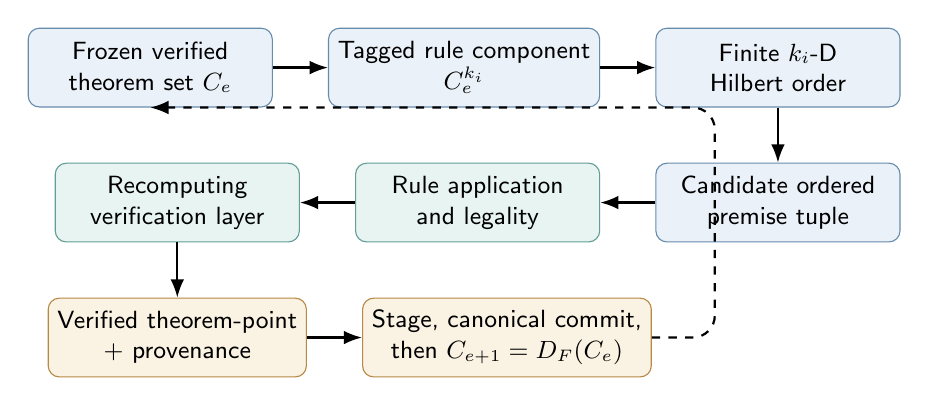
\begin{tikzpicture}[node distance=7mm and 7mm,>=Latex,font=\sffamily\small]
\tikzset{box/.style={draw=HilbertBlue!70,rounded corners=4pt,fill=SoftBlue,minimum width=3.1cm,minimum height=1.0cm,align=center},
         gate/.style={draw=HilbertTeal!75,rounded corners=4pt,fill=SoftTeal,minimum width=3.1cm,minimum height=1.0cm,align=center},
         outputbox/.style={draw=HilbertGold!80,rounded corners=4pt,fill=SoftGold,minimum width=3.1cm,minimum height=1.0cm,align=center}}
\node[box] (c) {Frozen verified\\theorem set $C_e$};
\node[box,right=of c] (rule) {Tagged rule component\\$C_e^{k_i}$};
\node[box,right=of rule] (hilb) {Finite $k_i$-D\\Hilbert order};
\node[box,below=of hilb] (tuple) {Candidate ordered\\premise tuple};
\node[gate,left=of tuple] (legal) {Rule application\\and legality};
\node[gate,left=of legal] (verify) {Recomputing\\verification layer};
\node[outputbox,below=of verify] (new) {Verified theorem-point\\+ provenance};
\node[outputbox,right=of new] (commit) {Stage, canonical commit,\\then $C_{e+1}=D_F(C_e)$};
\draw[->,thick] (c)--(rule);
\draw[->,thick] (rule)--(hilb);
\draw[->,thick] (hilb)--(tuple);
\draw[->,thick] (tuple)--(legal);
\draw[->,thick] (legal)--(verify);
\draw[->,thick] (verify)--(new);
\draw[->,thick] (new)--(commit);
\draw[->,thick,dashed,rounded corners=8pt] (commit.east) -- ++(.8,0) |- (c.south);
\end{tikzpicture}
\caption{One frozen theorem-discovery epoch.  Hilbert order schedules candidate inference addresses; verification alone licenses theorem-points.}
\label{fig:pipeline}
\end{figure}}

\newcommand{\CoproductFigure}{%
\begin{figure}[H]
\centering
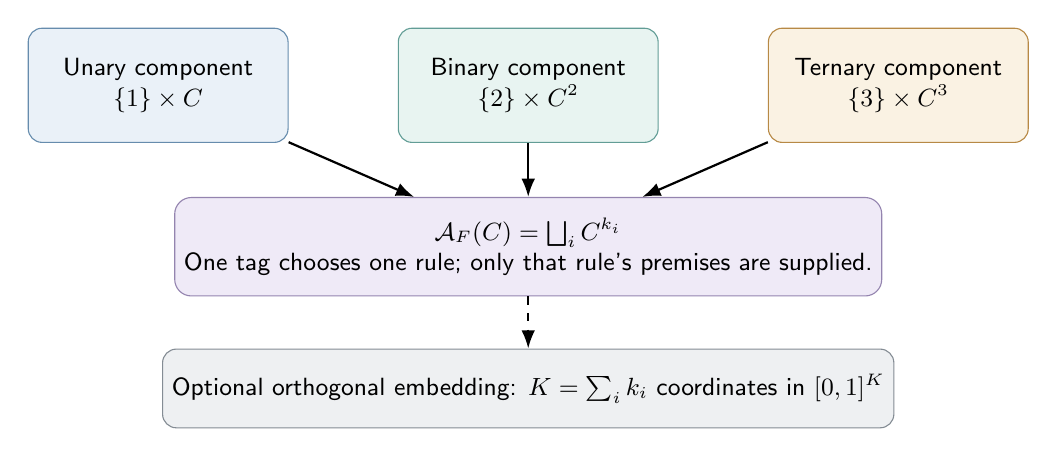
\begin{tikzpicture}[font=\sffamily\small,>=Latex]
\node[draw=HilbertBlue!70,fill=SoftBlue,rounded corners=5pt,minimum width=3.3cm,minimum height=1.45cm,align=center] (u) at (-4.7,1.7) {Unary component\\$\{1\}\times C$};
\node[draw=HilbertTeal!75,fill=SoftTeal,rounded corners=5pt,minimum width=3.3cm,minimum height=1.45cm,align=center] (b) at (0,1.7) {Binary component\\$\{2\}\times C^2$};
\node[draw=HilbertGold!80,fill=SoftGold,rounded corners=5pt,minimum width=3.3cm,minimum height=1.45cm,align=center] (t) at (4.7,1.7) {Ternary component\\$\{3\}\times C^3$};
\node[draw=HilbertPurple!70,fill=SoftPurple,rounded corners=6pt,minimum width=8.5cm,minimum height=1.25cm,align=center] (cop) at (0,-.35) {$\mathcal A_F(C)=\bigsqcup_i C^{k_i}$\\One tag chooses one rule; only that rule's premises are supplied.};
\node[draw=HilbertGray!70,fill=SoftGray,rounded corners=5pt,minimum width=8.5cm,minimum height=1.0cm,align=center] (amb) at (0,-2.15) {Optional orthogonal embedding: $K=\sum_i k_i$ coordinates in $[0,1]^K$};
\draw[->,thick] (u)--(cop);
\draw[->,thick] (b)--(cop);
\draw[->,thick] (t)--(cop);
\draw[->,thick,dashed] (cop)--(amb);
\end{tikzpicture}
\caption{The coproduct keeps rule-specific argument coordinates from interfering.  The sum of arities is an ambient embedding dimension, not the intrinsic dimension of every inference.}
\label{fig:coproduct}
\end{figure}}

\newcommand{\HilbertTwoDFigure}{%
\begin{figure}[H]
\centering
\begin{tikzpicture}
\begin{axis}[
  width=.82\textwidth,height=.65\textwidth,
  axis equal image,
  xlabel={Premise-slot coordinate 1},ylabel={Premise-slot coordinate 2},
  xmin=-.5,xmax=15.5,ymin=-.5,ymax=15.5,
  grid=both,major grid style={draw=gray!18},
  tick label style={font=\small},label style={font=\small\sffamily},
  title={Finite 2D Hilbert approximant: 256 cells},title style={font=\sffamily\bfseries}
]
\addplot[HilbertBlue,very thick] table[x index=1,y index=2] {hilbert2d.dat};
\addplot[only marks,mark=*,mark size=2.2pt,HilbertTeal] coordinates {(0,0) (15,0)};
\node[anchor=south west,font=\small\sffamily] at (axis cs:0,0) {start};
\node[anchor=south east,font=\small\sffamily] at (axis cs:15,0) {end};
\end{axis}
\end{tikzpicture}
\caption{Vector-rendered two-dimensional finite Hilbert traversal.  Consecutive cells are face-adjacent, so a local move changes exactly one premise-slot rank by one unit.}
\label{fig:hilbert2d}
\end{figure}}

\newcommand{\HilbertThreeDFigure}{%
\begin{figure}[H]
\centering
\begin{tikzpicture}
\begin{axis}[
  width=.86\textwidth,height=.68\textwidth,
  view={42}{24},
  xlabel={Premise slot 1},ylabel={Premise slot 2},zlabel={Premise slot 3},
  xmin=-.2,xmax=3.2,ymin=-.2,ymax=3.2,zmin=-.2,zmax=3.2,
  grid=major,
  tick label style={font=\scriptsize},label style={font=\small\sffamily},
  title={Finite 3D Hilbert approximant: 64 cells},title style={font=\sffamily\bfseries}
]
\addplot3[HilbertBlue,very thick] table[x index=1,y index=2,z index=3] {hilbert3d.dat};
\end{axis}
\end{tikzpicture}
\caption{Vector-rendered three-dimensional finite Hilbert traversal for a ternary rule component.}
\label{fig:hilbert3d}
\end{figure}}

\newcommand{\HilbertTitleMotif}{%

\begin{tikzpicture}[scale=.42]
  \draw[HilbertBlue,line width=1.4pt] (0,0)--(0,1)--(1,1)--(1,0)--(2,0)--(3,0)--(3,1)--(2,1)--(2,2)--(3,2)--(3,3)--(2,3)--(2,2)--(1,2)--(1,3)--(0,3)--(0,2)--(1,2)--(1,1);
\end{tikzpicture}}


% Stable navigation helpers. Force enough room before headings so
% hyperref anchors cannot be stranded on the preceding page.
\pretocmd{\section}{\Needspace{6\baselineskip}}{}{}
\pretocmd{\subsection}{\Needspace{4\baselineskip}}{}{}
\newcommand{\tocsection}[2]{%
  \Needspace{6\baselineskip}%
  \phantomsection
  \addcontentsline{toc}{section}{#1}%
  \section*{#1}%
  \label{#2}%
}
\newcommand{\tocsubsection}[2]{%
  \Needspace{4\baselineskip}%
  \phantomsection
  \addcontentsline{toc}{subsection}{#1}%
  \subsection*{#1}%
  \label{#2}%
}
\bookmarksetup{open,numbered}
\begin{document}
\begin{titlepage}
\thispagestyle{empty}
\centering
\vspace*{1.0cm}
{\HilbertTitleMotif\par}
\vspace{0.8cm}
{\sffamily\bfseries\fontsize{26}{31}\selectfont\color{HilbertBlue} Hilbert Space Filling Curve-Style\\Theorem Search\par}
\vspace{0.55cm}
{\Large A Mathematical Specification, Constrained-Search Study,\\and Research Program\par}
\vspace{0.85cm}
{\large\bfseries Version 0.5.3\par}
{\large August 7, 2026\par}
\vspace{0.9cm}
{\Large Brian Tenneson\par}
\vfill
\begin{tcolorbox}[width=.88\textwidth,colback=SoftBlue,colframe=HilbertBlue!70,arc=3mm,boxrule=.7pt]
\textbf{Research status:} expanded theoretical edition. The paper separates settled mathematical facts from open conjectures and experimental hypotheses.\\[2mm]
\textbf{Reader goal:} the paper is intended to be readable without requiring a second Tenneson manuscript beside it. Essential proof-theoretic vocabulary is restated locally and collected in the glossary appendix.\\[2mm]
\textbf{Scope:} the password-like examples are abstract constrained-search models. No credential-recovery implementation, operational attack procedure, rate-limit bypass, or deployment guidance is supplied.\\[2mm]
\textbf{Version 0.5.3:} navigation and typesetting correction. Numbered section and subsection headings now match the table of contents; top-level TOC entries use leaders to visible page numbers; the OEIS sequence examples are comma-separated; stale internal version references are removed; the long research question in Section 16 is reflowed within the text block; and the public source citations remain fixed to immutable GitHub copies.
\end{tcolorbox}
\vfill
{\small\sffamily This PDF was compiled from the reconstructed LaTeX source and re-rendered for visual verification.\par}
\end{titlepage}

% Physical page 1 is the title page. Keep printed and PDF-viewer page numbers aligned.
\setcounter{page}{2}
\tableofcontents
\clearpage

\tocsection{Abstract}{abstract}

This document specifies and implements a budgeted theorem-discovery method in which finite arbitrary-dimensional Hilbert-style traversals order candidate inference applications. For a frozen verified theorem set $C$ and a $k$-ary rule, the executable traverses a power-of-two grid of ranks in the frozen theorem list, which is sorted by WFF line number. Different inference rules live in a tagged coproduct, so arguments belonging to unrelated rules are not forced into one meaningless Cartesian product. Every accepted conclusion is stored with proof provenance and must pass a separate recomputing verification layer.

The document also develops an explicit rational-address layer from Brian Tenneson's surjection from the positive natural numbers onto the rationals, its least-preimage section, recursive tuple pairing, and a derived line numbering of rational $n$-cubes. A crucial implementation clarification is that these rational coordinates are global addresses and provenance in the current code; they do not yet determine the Hilbert metric. The implementation is a tested research prototype and forward consequence enumerator, not a decision procedure for ZFC and not yet a production Metamath prover.

\tocsection{The 135-Year Jigsaw: Where This Paper Fits}{historical-jigsaw}

\HistoryJigsawFigure

\textbf{1891 - Hilbert curve.} Hilbert published ``Ueber die stetige Abbildung einer Linie auf ein Flaechenstueck'' in \emph{Mathematische Annalen} 38, pp.~459--460. The original construction is two-dimensional; the arbitrary-dimensional Hilbert traversals used in this paper are later generalizations inspired by Hilbert, not a construction Hilbert himself wrote down \cite{hilbert1891}.

\textbf{1928 - Entscheidungsproblem.} Hilbert and Ackermann's \emph{Grundzuege der theoretischen Logik} formulated the decision problem for first-order logic: is there a general effective procedure that determines whether a given formula is provable / logically valid? This was not specifically a request for a ZFC theorem decider \cite{hilbertackermann1928}.

\textbf{1930-1931 - Goedel.} Goedel's 1930 completeness theorem showed that every logically valid first-order formula is provable in a complete proof calculus; this is a positive proof-enumeration result, not a terminating decision algorithm. His 1931 incompleteness theorems then showed that sufficiently strong, consistent, effectively axiomatized theories containing arithmetic cannot settle every sentence and cannot, under the usual hypotheses, prove their own consistency. His 1931 paper explicitly discusses \emph{Principia Mathematica} and Zermelo-Fraenkel-style set theory \cite{godel1930,godel1931}.

\textbf{1936 - Church.} Church proved that the general Entscheidungsproblem is unsolvable: there is no effective procedure that always terminates with the correct yes/no answer for arbitrary first-order validity \cite{church1936,churchnote1936}.

\textbf{1936/1937 - Turing.} Turing independently made ``effective procedure'' mathematically precise with his machine model and again obtained a negative solution to the Entscheidungsproblem. The work was written in 1936 and published in the \emph{Proceedings of the London Mathematical Society} in 1937 \cite{turing1936,sep2026}.

\textbf{What remains.} For ordinary effective proof calculi, theoremhood remains positively enumerable (semi-decidable): proofs are finite objects, so a fair enumeration can eventually find a proof that exists. What cannot be demanded in general is a finite stopping time that correctly declares every non-theorem. This paper is about scheduling that surviving positive search problem under budgets.

\textbf{Do the 2026 arithmetic.} The Hilbert curve is 135 years old (2026--1891). The Hilbert--Ackermann Entscheidungsproblem formulation is 98 years old (2026--1928). Goedel incompleteness is 95 years old (2026--1931). Church's and Turing's decisive computability results are 90 years old measured from 1936 (2026--1936).

\tocsection{Corrections and scope clarifications}{corrections-v030}
\begin{itemize}
\item The continuous limiting Hilbert curve is onto the full cube, hence onto every rational point in it. The executable algorithm, however, uses finite discrete Hilbert approximants. It visits grid cells exactly; it does not literally wait to hit arbitrary rational points of the limiting curve.
\item Theorem identity, proof identity, and inference address are different objects. A WFF may be assigned a rational coordinate, and each candidate $k$-premise inference has a $k$-dimensional rational address, but a theorem can have many proofs and many inference histories. Trusted theorem identity remains the WFF line plus a verified certificate/provenance record.
\item The current Hilbert scheduler traverses ranks in the frozen theorem list. Tenneson rational $n$-cube coordinates are recorded as global addresses/provenance; they are not yet the metric that determines Hilbert adjacency. This is the most important implementation-level correction to the earlier exposition.
\item For a formal system whose rules are actual computable partial functions of $k$ explicit premises, rule arity $k$ supplies the action dimension. For Metamath-style schemas, unification, substitutions, side conditions, and other independently variable choices may require additional coordinates. Arity alone is not automatically sufficient in a production ATP.
\item The toy verifier is separate from the search scheduler and recomputes rule applications, but it shares the same rule implementation. Calling it an ``independent verifier'' in the strong production-kernel sense was too strong. The present paper therefore calls it a separate recomputing verification layer.
\item The completeness statement is a forward-saturation result under finite-rule, effective, fair-enumeration hypotheses. It is not a total decision procedure and does not by itself establish completeness of a future Metamath adapter.
\end{itemize}

\section{Prior-art search result: no direct precedent located}\label{sec:prior-art}
A targeted literature search performed through August 7, 2026 found no published paper that directly uses a Hilbert space-filling curve or finite Hilbert order as the search scheduler over proof-theoretic inference addresses in automated theorem proving. Searches included combinations of ``Hilbert curve,'' ``space-filling curve,'' ``proof search,'' ``automated theorem proving,'' ``automated reasoning,'' ``proof theory,'' SAT, SMT, and formal verification across general web search and scholarly sources. This is a negative search result, not proof that no obscure precedent exists.

The neighboring literatures are real but distinct. Hilbert orders are used for locality-preserving multidimensional indexing, data mining, rendering, robotics, coverage, and other search/linearization problems \cite{skilling2004,haverkort2017,joshi2019,wakode2022,bohm2020,gotsman1996}. Modern ATP work uses machine-learned ranking, proof-structure analysis, and many other search orderings \cite{faerber2021,wernhard2024}. In 2026, Bryant et al.~reported an Isabelle/HOL autoformalization of Munkres topology that includes a space-filling-curve theorem, but the curve is something proved inside the formalization, not the mechanism used to search for proofs \cite{bryant2026}. A 2025 agentic Lean framework is named \emph{Hilbert}, but its name is unrelated to Hilbert space-filling curves \cite{varambally2025}. The careful novelty statement is therefore: to the best of the targeted search reported here, no direct precedent was located for Hilbert-order scheduling of ATP inference-address spaces.

\small
\begin{longtable}{@{}>{\raggedright\arraybackslash}p{0.22\textwidth}>{\raggedright\arraybackslash}p{0.34\textwidth}>{\raggedright\arraybackslash}p{0.36\textwidth}@{}}
\toprule
\textbf{Literature area} & \textbf{What exists} & \textbf{Relation to this project} \\
\midrule
\endhead
\bottomrule
\endlastfoot
Arbitrary-dimensional Hilbert algorithms & Butz, Skilling, and Haverkort give algorithms or systematic traversals for Hilbert-type curves in arbitrary finite dimension. & Directly supports the $k$-dimensional rule-component cursor. It does not supply an ATP interpretation. \\
Robotic coverage and exploration & Hilbert and other space-filling curves have been used to cover physical regions, including online obstacle avoidance. & Closest operational analogy: a path orders exhaustive visits. The searched objects here are premise tuples, not physical cells. \\
Multidimensional indexing and sampling & Space-filling curves linearize high-dimensional data while retaining locality approximately. & Supports the idea of reducing a multidimensional inference-address space to a one-dimensional schedule. \\
Formalization of space-filling curves & The space-filling-curve theorem itself has been formalized in proof assistants as part of larger topology developments. & The curve is the object being proved about, not the mechanism used to search for proofs. \\
Theorem provers named ``Hilbert'' & A 2025 agentic Lean framework is named Hilbert and recursively decomposes goals. & The name is unrelated to Hilbert space-filling curves; it is not prior art for this scheduling construction. \\
Direct ATP/proof-theory use located & No publication was located that uses a Hilbert/space-filling curve to enumerate tagged inference-rule premise tuples or to certify completed proof-search coverage. & This is a literature-search result, not a proof of novelty. A formal novelty claim requires a broader systematic search and expert review. \\
\end{longtable}
\normalsize

\section{The construction in one sentence}\label{sec:one-sentence}
\textbf{Use a finite $k$-dimensional Hilbert order to enumerate every ordered $k$-tuple of currently verified theorems for each $k$-ary inference rule; keep different rules in a tagged coproduct so their arguments do not form meaningless Cartesian products; verify every new conclusion; repeat with the enlarged theorem set under an explicit expansion budget.}

\PipelineFigure

\section{Mathematical foundation}\label{sec:math-foundation}
\subsection{Tenneson's explicit enumeration of the rationals}\label{subsec:rationals}
The symbols $\operatorname{A002260}$ and $\operatorname{A004736}$ below are identifiers from the \emph{On-Line Encyclopedia of Integer Sequences} (OEIS), not notation introduced in this paper or in Reference~\cite{tennesonNQ}. OEIS A002260 is the sequence $1,1,2,1,2,3,\ldots$, while OEIS A004736 is the corresponding row-reversed sequence $1,2,1,3,2,1,\ldots$ \cite{oeisA002260,oeisA004736}. The OEIS entries themselves attribute the following closed forms to Brian Tenneson (2003) \cite{oeisA002260,oeisA004736}.

Let $\langle x\rangle=\lfloor x+\tfrac12\rfloor$. With $t=\langle\sqrt{2m}\rangle$,
\[
\operatorname{A002260}(m)=\frac{2m+t-t^2}{2},
\qquad
\operatorname{A004736}(m)=\frac{2-2m+t+t^2}{2}.
\]
Reference~\cite{tennesonNQ} develops these coordinates into the explicit surjection used here. That later manuscript is distinct from the OEIS entries themselves. Its surjection $r:\mathbb N_+\twoheadrightarrow\mathbb Q$ is
\[
r(n)=(-1)^n\frac{\operatorname{A002260}(\lfloor n/2\rfloor)}{\operatorname{A004736}(\lfloor n/2\rfloor)}.
\]
For a reduced rational $p/q$ with $q\ge1$, the least-preimage section $s$ satisfies
\[
r\!\left(s\!\left(\frac pq\right)\right)=\frac pq.
\]
The implementation uses the two polynomial branches developed and proved in Tenneson's public manuscript \cite{tennesonNQ}.

\subsection{From \texorpdfstring{$\mathbb Q$}{Q} to \texorpdfstring{$\mathbb Q\cap[0,1]$}{Q intersect [0,1]}}\label{subsec:unit-interval}
A useful explicit transport preserves rationality and produces a canonical least line. Reserve line $1$ for the endpoint $1$. For $n\ge2$, set
\[
u(1)=1,
\qquad
u(n)=\frac{|r(n-1)|}{1+|r(n-1)|}.
\]
Then $u:\mathbb N_+\twoheadrightarrow\mathbb Q\cap[0,1]$. For $0\le q<1$, solve $q=t/(1+t)$ as $t=q/(1-q)$ and define
\[
u^{-1}_{\min}(q)=s\!\left(\frac{q}{1-q}\right)+1,
\qquad
u^{-1}_{\min}(1)=1.
\]
Because Tenneson's positive occurrence of a nonzero magnitude precedes its negative occurrence, this section returns the least line of the transported unit-interval enumeration.

\subsection{One line number for a rational \texorpdfstring{$n$}{n}-cube point}\label{subsec:ncube}
Use Tenneson's pairing polynomial
\[
\pi(a,b)=\frac{(a+b-1)(a+b-2)}{2}+a.
\]
Recursively pairing $n$ positive indices produces a bijection
\[
\pi_n:\mathbb N_+^n\longrightarrow\mathbb N_+.
\]
Decoding one line and applying $u$ coordinatewise gives an explicit surjection
\[
R_n:\mathbb N_+\twoheadrightarrow(\mathbb Q\cap[0,1])^n.
\]
Applying the unit-interval section coordinatewise and pairing the resulting indices gives a right inverse $S_n$, so
\[
R_n\bigl(S_n(q_1,\ldots,q_n)\bigr)=(q_1,\ldots,q_n).
\]

\subsection{WFF line numbers as distinct rational points}\label{subsec:wff-lines}
A merely surjective map may assign several formulas to the same rational coordinate. Formula identity must therefore remain the WFF/G\"odel line number. For geometry, use the injective map
\[
\iota(g)=\frac{g}{g+1},\qquad g=0,1,2,\ldots
\]
An ordered premise tuple with WFF lines $(g_1,\ldots,g_k)$ may be represented by the rational point $(\iota(g_1),\ldots,\iota(g_k))$, and Tenneson's least-preimage machinery can assign a canonical global natural-number line to that rational tuple. In the current implementation this is an address/provenance layer. The actual finite Hilbert traversal operates on the rank tuple $(j_1,\ldots,j_k)$ of those formulas in the WFF-line-sorted frozen theorem list. A future experiment may test Hilbert geometry built directly from a more semantically meaningful rational embedding. For effective WFF enumeration and its relation to proof search, see \cite{proofhorizon}.

\section{Why the search space is a coproduct}\label{sec:coproduct}
Let the rules be $r_1,\ldots,r_m$ with arities $k_1,\ldots,k_m$. For a frozen theorem set $C$, the intrinsic inference-address space is
\[
\mathcal A_F(C)=\bigsqcup_{i=1}^{m} C^{k_i}.
\]
A point is not an untagged tuple from one enormous product. It is a tagged object $(i;a_1,\ldots,a_{k_i})$ saying exactly which rule and which ordered premises are being tested. The optional ambient orthogonal dimension is $K=\sum_i k_i$. $K$ is useful for a geometric embedding, but the engine traverses each rule component at its own intrinsic dimension.

\CoproductFigure

\section{Finite Hilbert approximants}\label{sec:finite-hilbert}
At the start of epoch $e$, freeze the verified theorem list $C_e=(\theta_0,\ldots,\theta_{M-1})$, sorted by WFF line number. Choose $p=\lceil\log_2 M\rceil$ and $N=2^p$. A rule of arity $k$ receives a discrete $k$-dimensional Hilbert-style bijection. Hilbert's 1891 paper described the two-dimensional curve; arbitrary-dimensional discrete algorithms are later generalizations, including work by Butz, Skilling, and Haverkort \cite{butz1969,butz1971,skilling2004,haverkort2017}.
\[
H_{k,p}:\{0,\ldots,N^k-1\}\longrightarrow\{0,\ldots,N-1\}^k.
\]
A Hilbert step $h$ decodes to a coordinate tuple $(j_1,\ldots,j_k)$. If every $j_t<M$, it denotes the ordered premise tuple $(\theta_{j_1},\ldots,\theta_{j_k})$. Coordinates at least $M$ are padding. Padding allows an exact power-of-two Hilbert grid without duplicating valid tuples. Every valid ordered tuple in $C_e^k$ is visited exactly once in a completed rule-component pass.

\HilbertTwoDFigure

\section{Straight motion, turning, and changing rules}\label{sec:motion}
The discrete Hilbert path gives the geometric language an exact computational meaning. Straight motion means consecutive Hilbert steps continue to change the same coordinate axis: the same premise slot is varied while the other slots remain locally fixed. A turn within one rule component means the changed axis switches, so a different premise position is varied. A coproduct turn means the scheduler changes to a different tagged inference rule. In dimension $k$ there are $2k$ signed axis directions; excluding immediate reversal leaves $2k-1$ local nonreverse choices.

\section{The probe and theorem-points}\label{sec:probe}
The probe is not merely the current Hilbert coordinate. It is the complete monotone verified search state: theorem database, proof/provenance forest, unfinished rule cursors, current resolution, Hilbert step, remaining budgets, and append-only event history. For a particular theorem, the relevant proof is the predecessor subgraph inside that forest.

A candidate formula becomes a trusted theorem record only after a proof certificate is accepted by the recomputing verifier layer. The stored object includes the WFF line, formula, certificate, rule name, premise lines, discovery epoch, and provenance address. Because the prototype verifier reuses the same rule implementation as the formal-system object, it is a separation-of-responsibilities check rather than a fully independent production kernel.

\section{Frozen epochs and completeness}\label{sec:frozen-epochs}
Define the direct-consequence operator
\[
D_F(C)=C\cup\left\{r_i(a_1,\ldots,a_{k_i}):
(a_1,\ldots,a_{k_i})\in C^{k_i},\ r_i\text{ is defined}\right\}.
\]
During one epoch, every premise comes from the same frozen $C_e$. Novel verified conclusions are staged and committed only after the pass ends. If every rule component completes, every rule is a computable finite-arity partial function on explicit premises, and the verifier accepts exactly the legal consequences, then $C_{e+1}=D_F(C_e)$. Repeated fair complete epochs enumerate the deductive closure generated by those rules. This does not yet cover a real Metamath search until independently variable substitutions, unification choices, and side conditions have also been made part of the enumerable action space.

\section{Budgets, interruption, and what Hilbert order can actually change}\label{sec:budgets}
One expansion is one attempted inference-rule application on one valid decoded premise tuple. Address visits are counted separately because a padded power-of-two grid may include cells that do not decode to current theorem indices. For $M$ frozen theorems, the exact valid expansion count of a completed epoch is
\[
E(M)=\sum_i M^{k_i}.
\]
With $N=2^{\lceil\log_2 M\rceil}$, the total Hilbert address visits are
\[
A(M)=\sum_i N^{k_i}.
\]
For $M>1$, $M\le N<2M$, so a $k$-ary component visits $N^k<2^kM^k$ grid cells. The power-of-two embedding can therefore add padding overhead. It does not reduce the exhaustive candidate count.

This point deserves emphasis because it controls the interpretation of every later application. Hilbert order changes a schedule; it does not manufacture a smaller finite set. Any practical gain must therefore arise from visitation order under interruption, locality in the representation, cache or verification effects, adaptive allocation, or a downstream policy that exploits the order.

An interrupted run should report what it actually covered. A useful interruption certificate records valid expansions, padding visits, verifier calls, new theorem records, component cursor positions, completed resolution levels, and whether the epoch completed. A finite unsuccessful run remains an incomplete search, not a refutation and not evidence of independence.

\subsection{Why interruption makes ordering scientifically meaningful}\label{subsec:interruption}
If every candidate will eventually be visited and all candidates have equal cost, two complete exhaustive schedules have the same terminal coverage. Their difference appears before completion. Let $B$ be a finite budget. A schedule $\sigma$ induces a prefix
\[
P_B(\sigma)=\{\sigma(1),\ldots,\sigma(B)\}.
\]
The scientific question is therefore not whether Hilbert order can change the cardinality of the completed search, but whether $P_B(\sigma_H)$ has better properties than the corresponding prefix of a matched baseline. Those properties may include target probability mass, geometric coverage, verified theorem yield, or useful intermediate lemmas.

\subsection{Coarse-to-fine coverage}\label{subsec:coarse-fine}
A natural anytime variant completes a coarse finite Hilbert approximant before refining the grid. At level $m$, the unit cube is partitioned into dyadic cells of side $2^{-m}$. Completing level $m$ gives a global coverage statement at that scale. Refinement then replaces each coarse cell by smaller cells and repeats. The attraction is not that the method knows where the target is, but that an unknown stopping time does not automatically strand the search in one narrow lexicographic corner.

\begin{tcolorbox}[colback=SoftGold,colframe=HilbertGold!80,arc=2mm,boxrule=.6pt,title={Interpretive rule}]
A Hilbert schedule is interesting only relative to a representation. If nearby coordinates do not encode anything relevant to discovery, locality preservation is merely geometric decoration.
\end{tcolorbox}

\section{Password-like hidden-target search as a controlled model problem}\label{sec:hidden-target}
Password-like search is used here as an abstract hidden-target model, not as an operational credential-recovery recipe. It is valuable precisely because the amount of prior structure can be varied cleanly. The hidden string plays the role of an unknown target; the search procedure plays the role of a search party; a verifier reports whether a tested candidate is the target. In a physical analogy, known constraints are terrain information: a boat searches water rather than land, and a terrestrial search party does not waste its budget traversing an ocean.

The analogy should not be pushed too far. Real authentication systems deliberately impose rate limits, lockouts, cryptographic hashing, access controls, and other defenses. The mathematical model below studies finite constrained search in the abstract and supplies no method for defeating those controls.

\subsection{Case I: no informative structure}\label{subsec:no-information}
Let $P$ be a finite candidate set with $|P|=N$, and suppose exactly one candidate $p^*$ is the target. Assume $p^*$ is uniformly distributed and testing a candidate reveals only success or failure. Any deterministic nonrepeating exhaustive procedure induces a permutation
\[
p_1,p_2,\ldots,p_N.
\]
This includes lexicographic enumeration, breadth-first enumeration under a chosen tree, a random permutation fixed in advance, and a Hilbert-derived order after an arbitrary embedding.

\begin{theorem}[No-information ordering theorem]
Under the assumptions above, every fixed nonrepeating exhaustive ordering has expected discovery position $(N+1)/2$.
\end{theorem}
\begin{proof}
Each position $j$ contains the target with probability $1/N$. Therefore
\[
\mathbb E[T]=\frac1N\sum_{j=1}^{N}j=\frac{N+1}{2}.
\]
\end{proof}
The argument depends only on exchangeability of the target positions, not on the geometric name of the ordering.

This settles one tempting conjecture negatively: an arbitrary Hilbert embedding cannot, by itself, improve expected discovery in a completely uninformative uniformly distributed finite search. Geometry must earn its relevance.

\subsection{Case II: known hard conditions carve out feasible space}\label{subsec:hard-conditions}
Now suppose the target must satisfy known conditions $C_1,\ldots,C_n$. Define
\[
c_i(p)=\mathbf 1_{C_i}(p),\qquad c(p)=(c_1(p),\ldots,c_n(p))\in\{0,1\}^n.
\]
If all $n$ conditions are mandatory, the feasible set is
\[
P^*=\bigcap_{i=1}^{n}\{p\in P:c_i(p)=1\}.
\]
Candidates outside $P^*$ are known in advance to be inadmissible.

\begin{proposition}[Constraint reduction is scheduler-independent]
If every search method receives the same hard constraints, the reduction from $P$ to $P^*$ is attributable to constraint filtering, not to Hilbert ordering. A fair comparison must therefore compare schedulers on the same feasible set.
\end{proposition}
\begin{proof}
Membership in $P^*$ is defined before a visitation order is chosen. Any scheduler can restrict its domain to $P^*$. Thus the cardinality reduction $|P|\to|P^*|$ does not depend on which permutation of $P^*$ is subsequently used.
\end{proof}
This is the first important bridge back to theorem proving. Logical legality plays the same structural role as a hard constraint: it identifies candidate moves that are not admissible and therefore should not consume the same kind of search effort as legal candidates.

\subsection{Case III: constraints suggest coordinates, not merely exclusions}\label{subsec:features}
Binary feasibility is often only the beginning. A condition such as ``contains an uppercase symbol'' can be refined into a feature such as the number or positions of uppercase symbols. Abstractly, let
\[
\Phi:P^*\to\mathbb R^d,\qquad \Phi(p)=(f_1(p),\ldots,f_d(p)).
\]
The $f_i$ may describe length, class counts, transition statistics, repetition, syntactic categories, or other domain-appropriate properties. Hard constraints determine which candidates remain possible; the feature map determines which remaining candidates are near one another.

\begin{center}\bfseries
constraints define feasibility; features define locality; the scheduler defines visitation order.
\end{center}

If target probability varies smoothly or at least correlates locally with $\Phi$, then a locality-preserving traversal has something real to preserve. If not, the Hilbert curve is only a visually attractive permutation.

\subsection{Breadth-first search and Hilbert search use different primitive geometries}\label{subsec:bfs-v-hilbert}
Breadth-first search requires a rooted graph or tree and visits vertices in nondecreasing graph distance from the root. A string prefix tree, for example, naturally makes length a depth coordinate. Hilbert search instead requires a multidimensional embedding. The comparison is therefore between two notions of neighborhood:
\[
\text{tree proximity}\qquad\text{versus}\qquad\text{feature-space proximity}.
\]
Neither is automatically superior. If target likelihood is controlled mainly by tree depth, BFS may already possess the better geometry. If several interacting features matter and are poorly represented by depth, a multidimensional representation may expose structure that BFS ignores.

\subsection{The search-party picture}\label{subsec:search-party}
The hidden target may be imagined as an unaware object of search and the algorithm as a search party. In an unconstrained square, a path may sweep the whole region. If part of the square is forbidden terrain, the correct domain is no longer the whole square. The search should first respect the feasible region and only then ask how to traverse it. This is the conceptual role of password conditions, theorem-rule side conditions, obstacle fields in robotics, and admissibility constraints in many other search problems.

The analogy is useful because it separates two questions that are easy to blur: where may the search go? and in what order should it go there?

\section{From constrained hidden-target search back to automated theorem proving}\label{sec:back-to-atp}
Let $F=(x,y,z)$ be a formal system in the sense collected in Appendix A, let $\Gamma\subseteq y$ be a hypothesis set, and let $C\subseteq y$ be a finite frozen verified set. For a rule $r_i$ of arity $k_i$, a candidate premise address lies in $C^{k_i}$, and heterogeneous rules form the tagged coproduct
\[
\mathcal A_F(C)=\bigsqcup_i C^{k_i}.
\]
The password model suggests a three-layer decomposition for theorem search.

\textbf{Feasibility.} A candidate inference may be impossible because a rule is undefined on the selected premises, unification fails, a type or side condition fails, or a substitution is illegal. Such candidates are analogous to points on forbidden terrain.

\textbf{Representation.} Among legal inference candidates, one may define features: formula size, symbol profile, syntactic form, dependency history, proof depth, rule compatibility, learned embeddings, or other computable descriptors. These features define a candidate geometry.

\textbf{Scheduling.} Only after feasibility and representation are specified does Hilbert order enter. It linearizes the resulting multidimensional coordinates while attempting to preserve locality.

Thus the central research chain is
\[
\text{logical constraints}\to\text{legal region}\to\text{proof features}\to\text{geometry}\to\text{schedule}.
\]
This reframes the main risk of the current prototype. WFF-line rank is a stable address but need not be a good metric. A negative result for WFF-line geometry would therefore reject that representation, not automatically every possible Hilbert-ordered ATP.

\subsection{Hypotheses on the target theorem}\label{subsec:target-hypotheses}
The password analogy also suggests a controlled way to incorporate known properties of a desired theorem without confusing them with axioms. Suppose the target $\varphi$ is known to lie in a subclass $Y\subseteq y$: perhaps it has a designated syntactic form, concerns a differentiable function, contains particular symbols, belongs to a type class, or satisfies another mechanically checkable property. Such information is not an additional premise from which $\varphi$ may be proved. It is a search constraint on the target class.

That distinction matters. Adding a mathematical axiom changes $\operatorname{Con}_F(\Gamma)$. Adding a search filter does not. A target filter may change which proof attempts are prioritized or which terminal formulas count as relevant, but theoremhood remains governed by $F$ and $\Gamma$.

\begin{tcolorbox}[colback=SoftGold,colframe=HilbertGold!80,arc=2mm,boxrule=.6pt,title={Axiom versus search hypothesis}]
An axiom belongs to the hypothesis set $\Gamma$ and changes what is derivable. A search hypothesis is metadata about the desired target or promising candidates and changes only the search policy. Conflating the two would make the prover unsound.
\end{tcolorbox}

\subsection{A hybrid breadth/Hilbert architecture}\label{subsec:hybrid}
The password comparison suggests that Hilbert order need not replace breadth-first proof search. Let $L_m$ denote a derivational-depth layer or another breadth-controlled frontier. One may preserve the outer breadth discipline while using Hilbert order inside each layer. In that architecture, breadth controls vertical proof depth and Hilbert order controls horizontal locality among comparable inference candidates.

This hybrid is attractive because it permits a matched experiment: ordinary BFS and breadth-preserving Hilbert-BFS can share the same layers, legal candidates, verifier, and budget. Only the intra-layer visitation order changes.

\section{Short pseudocode for the theory}\label{sec:pseudocode}
The pseudocode is intentionally short. It is a mathematical bridge, not a credential-recovery implementation and not a production prover.
\begin{lstlisting}[style=hilbertcode,caption={Abstract constrained-search scheduler}]
INPUT: feasible-set test F, feature map Phi, verifier V, budget B

CANDIDATES := all abstract candidates admitted by F
EMBED each candidate by Phi
ORDER finite cells by a chosen Hilbert approximant

for candidate p in that scheduled order:
    if budget exhausted: return INTERRUPTED
    if V(p) succeeds: return FOUND
return EXHAUSTED
\end{lstlisting}

For theorem search the verifier has a stronger role: it does not merely recognize a hidden target; it certifies that a proposed conclusion follows by an allowed inference rule.
\begin{lstlisting}[style=hilbertcode,caption={Frozen-epoch Hilbert theorem search}]
C := verified hypotheses
repeat:
    freeze C
    NEW := empty
    for each tagged rule component:
        visit its legal premise addresses in Hilbert order
        apply the rule
        verify every proposed conclusion
        stage verified novel conclusions in NEW
    commit NEW only after the frozen epoch
    C := C union NEW
until budget exhausted, target verified, or a complete epoch adds nothing
\end{lstlisting}
The pseudocode exposes the separation of responsibilities: legality determines the feasible region; coordinates determine geometry; Hilbert order determines visitation; verification determines trust.

\section{Settled conjectures and resolved questions}\label{sec:settled}
This section records questions that no longer need conjectural status under the paper's stated model. Preserving them is useful because it shows which parts of the research program are mathematical facts and which remain empirical.

\subsection{Resolved: does Hilbert order reduce exhaustive candidate count?}
\textbf{Resolution: no.} For a frozen set of size $M$, a $k$-ary rule still has exactly $M^k$ ordered premise tuples. A Hilbert bijection changes their visitation order; power-of-two padding may increase address visits. Any advantage must therefore be a prefix, locality, interruption, or systems effect rather than a cardinality reduction.

\subsection{Resolved: does a complete finite Hilbert component miss valid tuples?}
\textbf{Resolution: no, under the stated bijection hypothesis.} If the finite Hilbert approximant is bijective on the padded grid, every valid tuple is visited exactly once. This is a coverage theorem, not a performance theorem.

\subsection{Resolved: what does a completed frozen epoch compute?}
\textbf{Resolution: the one-step direct-consequence closure.} Under effective finite-arity rules and exact verification, a completed epoch commits exactly $D_F(C)$. Repeated complete fair epochs positively enumerate $\operatorname{Con}_F(\Gamma)$.

\subsection{Resolved negatively: can arbitrary Hilbert ordering beat an uninformed uniform hidden-target search merely by reordering it?}
\textbf{Resolution: no.} The no-information ordering theorem in Section~\ref{subsec:no-information} gives expected discovery position $(N+1)/2$ for every fixed nonrepeating order. This negative result is important: it prevents the geometric metaphor from outrunning the information available to the search.

\subsection{Resolved: who gets credit for pruning hard constraints?}
\textbf{Resolution: the constraints.} If two schedulers receive the same hard constraints, both may restrict themselves to the same feasible set. Hilbert order should not be credited for candidate elimination performed before scheduling.

\section{Open conjectures: one research question per page}\label{sec:open-conjectures}
The conjectures below are intentionally separated from the settled results. Each is accompanied by its significance, reasons for and against, the author's expectation and preference, possible consequences, and a route toward resolution. ``Author preference'' is not evidence; it is disclosed because research programs are easier to evaluate when aspirations are distinguished from predictions.

\clearpage
\tocsubsection{Conjecture 1: Semantic-locality productivity}{conj1-heading}
\begin{conjecture}[Semantic-locality productivity]
Let a fixed formal library be equipped with a stable embedding whose local neighborhoods correlate positively with proof relevance. Under a fixed expansion budget, Hilbert traversal of the induced premise-coordinate space yields more verified novel theorems, or shorter time to a specified target proof, than lexicographic and uniformly random ordering on a nontrivial fraction of benchmark problems.
\end{conjecture}
\textbf{Why it matters.} This is the central performance conjecture. The mathematical construction already guarantees coverage under completed epochs; what is unknown is whether locality can improve useful prefixes of an interrupted search. If true, space-filling-curve geometry would become more than an indexing convenience: it would become a measurable proof-search heuristic.

\textbf{Why it might be true.} Proof-relevant formulas are often not isolated objects. They share symbols, subterms, types, dependencies, and derivational histories. If an embedding places such formulas near one another, then nearby premise tuples may share applicability patterns or produce families of related lemmas. Hilbert order could exploit that local correlation without requiring a globally accurate ranking model.

\textbf{Why it might be false.} Proof relevance may be too discontinuous. A decisive lemma can be syntactically remote from the goal, and useful premise combinations can involve formulas that are individually dissimilar. A learned best-first policy may also dominate any fixed locality-preserving traversal.

\textbf{Author expectation.} Plausible only after replacing arbitrary WFF-line rank by a structurally or learned meaningful embedding. The current line-rank geometry is not expected to be a strong test of the conjecture.

\textbf{Author preference.} True. A positive result would justify the geometric core of the project while still leaving room for hybrid learned policies.

\textbf{If true.} A natural corollary of the research program would be to study which formula features produce the strongest locality signal and whether Hilbert order is robust across theorem libraries.

\textbf{If false.} A carefully negative result would be valuable. It would suggest that proof relevance is not sufficiently local for this scheduler, or that locality must be exploited by a different mechanism.

\textbf{How to settle it.} Freeze a theorem library, verifier, hardware environment, target set, and expansion budget. Compare Hilbert, lexicographic, random, breadth-balanced, and learned controls over many targets. Report target success probability, expansions to proof, theorem yield, proof length, duplicate rate, and wall time.

\clearpage
\tocsubsection{Conjecture 2: Interruption robustness}{conj2-heading}
\begin{conjecture}[Interruption robustness]
If useful inference addresses occur in spatially clustered regions and stopping time is unknown in advance, a coarse-to-fine Hilbert schedule has lower expected uncovered-region radius at interruption, and more stable verified-theorem yield, than a one-direction lexicographic sweep with the same number of address visits.
\end{conjecture}
\textbf{Significance.} Real searches are often stopped by budgets rather than mathematical completion. A scheduler that degrades gracefully under interruption can be useful even when its completed exhaustive behavior is identical to a baseline.

\textbf{Why it might be true.} Coarse-to-fine traversal deliberately spreads early effort across the domain. Lexicographic order can spend a large prefix in one coordinate slab. If useful addresses cluster throughout the space rather than near the lexicographic origin, broader early coverage may reduce variance across unknown stopping times.

\textbf{Why it might be false.} Global coverage is not the same as useful coverage. If theorem-producing regions are concentrated near a simple boundary or if the baseline order accidentally aligns with the library's structure, coarse global sampling may waste budget.

\textbf{Author expectation.} The geometric coverage portion is expected to be easier to establish than the theorem-yield portion. The latter depends on the embedding.

\textbf{Author preference.} True in a qualified, benchmark-dependent sense rather than as a universal dominance theorem.

\textbf{Consequences.} A positive result would support interruption certificates and multiresolution scheduling as first-class ATP design features. A negative result would warn against confusing visually uniform coverage with proof productivity.

\textbf{Resolution path.} Measure both purely geometric coverage statistics and proof-search outcomes at many randomly selected interruption budgets. This separates the traversal property from the ATP property.

\clearpage
\tocsubsection{Conjecture 3: Representation dominance}{conj3-heading}
\begin{conjecture}[Representation dominance]
For a fixed budgeted theorem-search task, changing from an arbitrary address ordering to an embedding correlated with proof relevance produces a larger performance effect than changing among reasonable locality-preserving space-filling traversals while holding the embedding fixed.
\end{conjecture}
\textbf{Significance.} If true, the research priority shifts. The most important problem would not be choosing the perfect curve; it would be discovering the right geometry of proof space.

\textbf{Why it might be true.} Every locality-preserving traversal can preserve only the neighborhoods supplied to it. A bad metric makes good traversal behavior irrelevant. The password model makes this vivid: arbitrary coordinates do not create information.

\textbf{Why it might be false.} Different traversals can have materially different locality, boundary, anisotropy, and multiscale properties. A particular proof geometry might interact strongly with one traversal and poorly with another.

\textbf{Author expectation.} More likely true than false. The representation appears to be the largest scientific risk in the current prototype.

\textbf{Author preference.} Mildly true. It would simplify the program by focusing effort on representations while treating the Hilbert curve as a robust default scheduler rather than a sacred object.

\textbf{If true.} One research implication is to benchmark many embeddings before benchmarking many curves. Learned semantic coordinates, structural coordinates, and derivational coordinates become primary experimental variables.

\textbf{If false.} The traversal itself deserves deeper mathematical study, including alternative space-filling curves, anisotropic variants, and domain-specific path construction.

\textbf{How to settle it.} Use a factorial experiment: several embeddings crossed with several traversal families under identical budgets. Compare effect sizes attributable to representation and traversal.

\clearpage
\tocsubsection{Conjecture 4: Hybrid breadth-Hilbert advantage}{conj4-heading}
\begin{conjecture}[Hybrid breadth-Hilbert advantage]
There exist structured theorem families for which a breadth-preserving search that uses Hilbert ordering within comparable depth layers improves bounded target success or theorem yield over ordinary within-layer enumeration, while retaining the outer breadth discipline.
\end{conjecture}
\textbf{Significance.} This conjecture avoids a false choice between BFS and Hilbert search. Breadth-first search has a principled relationship to derivational depth; Hilbert order has a potential relationship to horizontal locality. A hybrid may exploit both.

\textbf{Why it might be true.} Within one breadth layer there can still be an enormous number of candidate inference tuples. Their internal order is not dictated by breadth itself. A locality-preserving schedule can therefore change finite-budget behavior without abandoning the layer structure.

\textbf{Why it might be false.} If useful proofs are dominated by a small number of high-value premises, learned ranking or conventional term indexing may overwhelm any geometric advantage. Hilbert overhead may also erase modest gains.

\textbf{Author expectation.} This is considered one of the more plausible ATP conjectures because it asks Hilbert order to solve a narrower problem than replacing BFS globally.

\textbf{Author preference.} True. It would make the proposal easier to integrate into existing provers as an internal scheduling policy rather than a wholesale architectural replacement.

\textbf{Consequences.} A positive result suggests a modular integration path. A negative result would narrow the plausible role of Hilbert traversal to non-breadth settings or specialized representations.

\textbf{Resolution path.} Implement matched BFS and BFS-with-Hilbert-intralayer ordering, with identical legal candidate sets and proof-depth policy. Compare across finite budgets and theorem families.

\clearpage
\tocsubsection{Conjecture 5: Constraint-induced hidden-target locality}{conj5-heading}
\begin{conjecture}[Constraint-induced hidden-target locality]
For some finite hidden-target search families, known target conditions induce quantitative features whose neighborhoods correlate with target probability strongly enough that a coarse-to-fine Hilbert schedule outperforms an equally constraint-aware locality-oblivious baseline under some finite budgets.
\end{conjecture}
\textbf{Significance.} This is the principal password-like conjecture. It asks whether prior conditions can do more than prune impossible candidates: can they help define a useful geometry among the candidates that remain?

\textbf{Why it might be true.} A binary condition can often be refined into quantitative structure. ``Has property $C_i$'' may correspond to counts, positions, distances, or pattern classes. If the target distribution is nonuniform across those features, local regions can carry different probability mass.

\textbf{Why it might be false.} Hard conditions may collapse every feasible candidate into the same coarse signature, leaving no useful within-region locality. Moreover, a probability-ranked method could exploit the same information more directly than Hilbert order.

\textbf{Author expectation.} True for specially constructed or naturally clustered target distributions; not expected as a universal statement about arbitrary strings.

\textbf{Author preference.} Scientifically neutral. A negative result would be almost as useful as a positive one because it would clarify that constraints and geometry are substantially independent.

\textbf{If true.} The hidden-target model becomes a laboratory for measuring how much locality is required before a space-filling schedule becomes useful. It would also motivate analogous feature construction for theorem search.

\textbf{If false.} The paper gains an important boundary result: pruning and locality should be treated as separate resources, and the existence of many known conditions does not imply that a Hilbert geometry is informative.

\textbf{How to settle it safely.} Use synthetic finite string sets or other noncredential hidden-target benchmarks with known probability distributions. Give every scheduler the same feasible set and features. Measure discovery probability before budget $B$. No live authentication system is required or appropriate.

\clearpage
\tocsubsection{Conjecture 6: Locality threshold}{conj6-heading}
\begin{conjecture}[Locality threshold]
For a fixed family of budgeted search problems and a fixed class of locality-preserving schedules, there is a measurable regime in which increasing correlation between geometric proximity and search relevance changes Hilbert ordering from statistically indistinguishable from uninformed baselines to detectably advantageous.
\end{conjecture}
\textbf{Significance.} The conjecture asks not merely whether locality matters, but how much locality is enough to justify geometric scheduling.

\textbf{Why it might be true.} At zero informative correlation, the no-information theorem gives no ordering advantage in the uniform model. At very strong correlation, contiguous exploration of high-value neighborhoods should plausibly matter. It is natural to ask whether an empirical transition can be measured between these extremes.

\textbf{Why it might be false.} There may be no sharp threshold, only a smooth and problem-specific continuum. Different budgets, dimensions, and cluster shapes may move the transition so much that a single useful threshold parameter does not exist.

\textbf{Author expectation.} A universal constant is not expected. A family-dependent threshold or response curve is considered plausible.

\textbf{Author preference.} True in the weaker family-dependent sense. Such a result would turn ``meaningful locality'' from rhetoric into a measurable design criterion.

\textbf{Consequences.} If measurable, the threshold could guide whether a proposed embedding is worth the cost of Hilbert scheduling. If not, embedding evaluation will require richer diagnostics than a single locality statistic.

\textbf{Resolution path.} Construct controlled benchmark families in which the correlation between distance and target/relevance value can be tuned continuously. Plot scheduler performance against the locality parameter and budget.

\section{Experimental hypotheses and the sgrpcl pilot}\label{sec:sgrpcl}
A concrete benchmark prediction should be labeled an experimental hypothesis rather than a mathematical conjecture.

\textbf{Pilot hypothesis.} In a frozen Predator/Metamath \texttt{sgrpcl} environment, a legal-first Hilbert-aware ordering of canonically addressed assertion applications requires fewer expansions to the first externally verified \texttt{sgrpcl} certificate than a matched dense-uniform legal-first control, conditional on both methods producing a certificate within the same declared budget. The Metamath formal environment is documented in \cite{metamath}; the relevant Predator reproducibility record is \cite{predatorrecord}.

The experiment should be preregistered as far as practical: theorem library hash, target, hardware, verifier, expansion definition, random seeds, timeout, memory limit, and all compared schedules. A crash, timeout, or failure to find the target is data. It should be reported rather than silently discarded.

The strongest result would not be a single dramatic success. It would be a reproducible distribution across multiple targets and budgets showing where Hilbert scheduling helps, hurts, or makes no detectable difference.

\section{Future work: from flat search domains to curved ones}\label{sec:future-curved}
The present construction deliberately stays in flat finite coordinate domains: products of finite rank sets, rational unit cubes, and Euclidean-style embeddings. That is already enough structure for a substantial ATP experiment. A natural next question is therefore left open rather than forced into the current paper:

\begin{tcolorbox}[colback=SoftBlue,colframe=HilbertBlue!70,arc=2mm,boxrule=.6pt,title={Leading question}]
\centering\Large\bfseries What happens when the search domain is a manifold rather than a Euclidean subset?
\end{tcolorbox}

If a future search space is modeled by a manifold $M$ with metric $g$, Euclidean distance would be replaced locally by the geometry induced by $g$, and shortest local motion would be described by geodesic distance $d_g$. A future analogue of the present scheduling problem could therefore begin with the deliberately schematic question
\[
\begin{aligned}
&\text{Can one construct } H:[0,1]\to M \text{ whose finite approximants}\\
&\text{give useful locality-preserving coverage relative to } d_g\text{?}
\end{aligned}
\]
This line is a research prompt, not a theorem asserted here. On a general manifold, topology, curvature, coordinate charts, boundaries, singularities, and global obstructions can matter. The phrase ``Hilbert curve on a manifold'' therefore requires definitions rather than analogy alone.

The conceptual motivation is broader than physics. Route planning, maze solving, robotic coverage, constrained optimization, hidden-target search, and theorem search can all be viewed as traversal problems on structured state spaces without being mathematically equivalent problems. Curved state spaces arise naturally in geometry, mechanics, statistics, optimization, and physics, but the underlying question is mathematical: what should replace a Euclidean Hilbert schedule when the geometry of admissible motion is itself non-Euclidean?

That question is intentionally deferred. The present paper's job is to make the flat-space construction precise enough to test.

\section{Discussion: what the paper now claims, and what it does not}\label{sec:discussion}
The paper makes a modest mathematical claim and a larger experimental proposal. The mathematical claim is that finite Hilbert-style traversals can be used as complete orderings of finite rule-specific premise grids, and that completed frozen epochs recover ordinary one-step forward consequence under the stated hypotheses. The experimental proposal is that useful coordinate geometry may improve finite-budget search prefixes.

The password-like model strengthens the proposal by supplying a negative control. When no informative structure exists, Hilbert order has no intrinsic expected-position advantage. When hard constraints exist, they reduce feasible space independently of the scheduler. Only when the representation contains useful locality does Hilbert scheduling acquire a plausible mechanism for advantage.

This three-stage distinction - no information, constraints, informative geometry - is the conceptual center of the revised paper. It prevents the space-filling curve from being treated as magic and turns the research program into a sequence of falsifiable questions.

\section{Conclusion}\label{sec:conclusion}
Hilbert's space-filling idea supplies a disciplined way to linearize multidimensional search coordinates. In theorem proving, the natural coordinates arise from rule-specific premise choices and possibly additional substitution or side-condition variables. The correct global action space is a tagged coproduct of those components, not an artificial product that supplies arguments to every rule simultaneously.

The revised analysis separates four layers that should remain distinct: logical consequence, feasibility, representation, and scheduling. Completed fair epochs preserve positive enumeration of consequence. Constraints remove impossible candidates. Feature maps define neighborhoods. Hilbert order determines which neighborhoods are visited early under a finite budget.

The password-like hidden-target model shows both the attraction and the limitation of the idea. Without information, Hilbert order is merely another permutation. With hard constraints, the search space can shrink, but the credit belongs to the constraints. With informative geometry, locality-preserving traversal becomes a genuine hypothesis to test.

The next decisive step is therefore empirical rather than rhetorical: freeze a formal environment, choose matched baselines, define budgets before running, and measure. A positive result would identify a new scheduling tool for ATP. A negative result would still sharpen our understanding of proof-space geometry. Either outcome advances the question.

\clearpage
\phantomsection
\addcontentsline{toc}{section}{References}
\label{references}
\begingroup\small\sloppy
\begin{thebibliography}{99}
\bibitem{tennesonNQ} Brian Tenneson. \emph{A Closed-Form Surjection from N onto Q --- With Its Pseudo-Inverse}. Version 2.2, July 17, 2026. Public manuscript, math.NT (Number Theory), GitHub repository \texttt{btenneson/pub}. \href{https://github.com/btenneson/pub/blob/23739bb3bd04be90ef26f33717ac65feb1407b3d/math.NT%20%E2%80%94%20Number%20Theory/A%20Closed-Form%20Surjection%20from%20N%20onto%20Q%20by%20Brian%20Tenneson%202.2.pdf}{Immutable PDF at commit \texttt{23739bb3}.}\ \href{https://btenneson.github.io/pub/papers/closed_form_surjection_n_to_q/}{Live article}.
\bibitem{proofhorizon} Brian Tenneson. \emph{The Universal Proof-Horizon Operator: From MIU and the nth Well-Formed Formula to ZFC, Predator, and Automated Logical Deciders}. Version 1.0, August 3, 2026. Public manuscript, math.LO (Logic), GitHub repository \texttt{btenneson/pub}. \href{https://github.com/btenneson/pub/blob/23739bb3bd04be90ef26f33717ac65feb1407b3d/math.LO%20%E2%80%94%20Logic/The%20Universal%20Proof-Horizon%20Operator%20by%20Brian%20Tenneson%201.0.pdf}{Immutable PDF at commit \texttt{23739bb3}.}\ \href{https://btenneson.github.io/pub/papers/universal_proof_horizon_operator/}{Live article}.
\bibitem{oeisA002260} OEIS Foundation Inc. \emph{The On-Line Encyclopedia of Integer Sequences}, A002260: ``Triangle read by rows: T(n,k) = k for n >= 1, k = 1..n.'' The entry attributes the displayed closed form to Brian Tenneson, Oct. 11, 2003. \url{https://oeis.org/A002260}
\bibitem{oeisA004736} OEIS Foundation Inc. \emph{The On-Line Encyclopedia of Integer Sequences}, A004736: ``Triangle read by rows: row n lists the first n positive integers in decreasing order.'' The entry attributes the displayed closed form to Brian Tenneson, Oct. 11, 2003. \url{https://oeis.org/A004736}
\bibitem{butz1969} Arthur R. Butz. Convergence with Hilbert's Space Filling Curve. \emph{Journal of Computer and System Sciences} 3(2), 1969. DOI: 10.1016/S0022-0000(69)80010-3. \url{https://doi.org/10.1016/S0022-0000(69)80010-3}
\bibitem{butz1971} Arthur R. Butz. Alternative Algorithm for Hilbert's Space-Filling Curve. \emph{IEEE Transactions on Computers} C-20(4), 424--426, 1971. DOI: 10.1109/T-C.1971.223258. \url{https://doi.org/10.1109/T-C.1971.223258}
\bibitem{skilling2004} John Skilling. Programming the Hilbert Curve. \emph{AIP Conference Proceedings} 707, 381--387, 2004. DOI: 10.1063/1.1751381. \url{https://doi.org/10.1063/1.1751381}
\bibitem{haverkort2017} Herman Haverkort. Sixteen Space-Filling Curves and Traversals for $d$-Dimensional Cubes and Simplices. arXiv:1711.04473. \url{https://arxiv.org/abs/1711.04473}
\bibitem{joshi2019} Anant A. Joshi, Maulik C. Bhatt, and Arpita Sinha. Modification of Hilbert's Space-Filling Curve to Avoid Obstacles: A Robotic Path-Planning Strategy. \emph{Indian Control Conference}, 2019. DOI: 10.1109/ICC47138.2019.9123166. \url{https://doi.org/10.1109/ICC47138.2019.9123166}
\bibitem{wakode2022} Ashay Wakode and Arpita Sinha. Space Filling Curves for Coverage Path Planning with Online Obstacle Avoidance. arXiv:2209.01426. \url{https://arxiv.org/abs/2209.01426}
\bibitem{bohm2020} Christian B\"ohm. Space-Filling Curves for High-Performance Data Mining. arXiv:2008.01684. \url{https://arxiv.org/abs/2008.01684}
\bibitem{bryant2026} Dustin Bryant, Jonathan Juli\'an Huerta y Munive, Cezary Kaliszyk, and Josef Urban. Munkres' General Topology Autoformalized in Isabelle/HOL. arXiv:2604.07455, 2026. \url{https://arxiv.org/abs/2604.07455}
\bibitem{varambally2025} Sumanth Varambally et al. \emph{Hilbert: Recursively Building Formal Proofs with Informal Reasoning}. arXiv:2509.22819, 2025. \url{https://arxiv.org/abs/2509.22819}
\bibitem{hilbert1891} David Hilbert. Ueber die stetige Abbildung einer Linie auf ein Flaechenstueck. \emph{Mathematische Annalen} 38 (1891), 459--460.
\bibitem{church1936} Alonzo Church. An Unsolvable Problem of Elementary Number Theory. \emph{American Journal of Mathematics} 58(2), 345--363, 1936.
\bibitem{turing1936} A. M. Turing. On Computable Numbers, with an Application to the Entscheidungsproblem. \emph{Proceedings of the London Mathematical Society}, Series 2, 42, 230--265, 1936/1937.
\bibitem{hilbertackermann1928} David Hilbert and Wilhelm Ackermann. \emph{Grundzuege der theoretischen Logik}. Springer, Berlin, 1928.
\bibitem{godel1930} Kurt Goedel. Die Vollstaendigkeit der Axiome des logischen Funktionenkalkuels. \emph{Monatshefte fuer Mathematik und Physik} 37, 349--360, 1930.
\bibitem{godel1931} Kurt Goedel. Ueber formal unentscheidbare Saetze der Principia Mathematica und verwandter Systeme I. \emph{Monatshefte fuer Mathematik und Physik} 38, 173--198, 1931. DOI: 10.1007/BF01700692.
\bibitem{churchnote1936} Alonzo Church. A Note on the Entscheidungsproblem. \emph{Journal of Symbolic Logic} 1(1), 40--41, 1936; correction 1(3), 101--102, 1936. DOI: 10.2307/2269326.
\bibitem{sep2026} Stanford Encyclopedia of Philosophy. \emph{The Church-Turing Thesis: The Rise and Fall of the Entscheidungsproblem; Alan Turing; Goedel's Incompleteness Theorems}. Accessed August 7, 2026.
\bibitem{gotsman1996} C. Gotsman and M. Lindenbaum. On the Metric Properties of Discrete Space-Filling Curves. \emph{IEEE Transactions on Image Processing} 5(5), 794--797, 1996. DOI: 10.1109/83.499920.
\bibitem{faerber2021} Michael Faerber, Cezary Kaliszyk, and Josef Urban. Machine Learning Guidance for Connection Tableaux. \emph{Journal of Automated Reasoning} 65, 287--320, 2021. DOI: 10.1007/s10817-020-09576-7.
\bibitem{wernhard2024} Christoph Wernhard and Wolfgang Bibel. Investigations into Proof Structures. \emph{Journal of Automated Reasoning} 68, Article 24, 2024. DOI: 10.1007/s10817-024-09711-8.
\bibitem{depths461} Brian Tenneson. \emph{Depths of Induction and Formalized Self-Awareness: Formal Systems, Inference Closure, Automated Theorem Proving, Simulations, and Self-Aware Structures}. Version 46.1, Corrected Edition, July 30, 2026.
\bibitem{metamath} Norman D. Megill and David A. Wheeler. \emph{Metamath: A Computer Language for Mathematical Proofs}. 2nd ed., Lulu Press, 2019. \url{https://us.metamath.org/downloads/metamath.pdf}
\bibitem{predatorrecord} Brian Tenneson. \emph{Predator 8.004 Experiment Record: prcom Calibration and sgrpcl Preprocessing}. Unpublished reproducibility log, run record dated August 3, 2026.
\end{thebibliography}
\endgroup

\clearpage
\tocsection{Appendix A. Glossary and formal-system conventions}{appendix-a}
This appendix is a local repository of definitions used by the paper. It is intentionally sufficient for reading the paper without consulting another manuscript. The notation follows the $xyz$ convention used in Tenneson's \emph{Depths of Induction and Formalized Self-Awareness}, Version 46.1, with minor prose adaptation for this paper \cite{depths461}.

\textbf{Definition 1 (xyz formal system).} A formal system is an ordered triple $F=(x,y,z)$ such that $x$ is a nonempty alphabet, $y$ is a set of finite strings over $x$ designated as well-formed formulas, and $z$ is a set of finitary inference rules on $y$. If $r$ takes $k$ ordered premises, its arity is $\operatorname{ar}(r)=k$.

\textbf{Symbols.} Elements of $x$.

\textbf{Well-formed formulas (WFFs).} Elements of $y$.

\textbf{Inference rules.} Elements of $z$. A $k$-ary rule may be regarded here as an effective partial operation on $y^k$ when the rule is not defined for every tuple.

\textbf{Definition 2 (Hypothesis or axiom set).} A set $\Gamma\subseteq y$ supplies the formulas available without prior derivation. The set $\Gamma$ is not one of the three coordinates of $F=(x,y,z)$ in this convention. Different hypothesis sets may therefore be studied over the same formal system.

\textbf{Definition 3 (Direct consequence).} Let $A\subseteq y$ and $\beta\in y$. Then $\beta$ is a direct consequence of $A$ if there exist $k\ge1$, a $k$-ary rule $r\in z$, and $(a_1,\ldots,a_k)\in A^k$ such that $r(a_1,\ldots,a_k)=\beta$.

\textbf{Definition 4 (Proof from $\Gamma$).} A proof from $\Gamma$ is a finite sequence $\pi=\langle\pi(1),\ldots,\pi(n)\rangle$ of WFFs such that each line is either a member of $\Gamma$ or a direct consequence of earlier lines. The proof length is $|\pi|=n$.

\textbf{Provability notation.} Write $\Gamma\vdash_F\psi$ when some proof from $\Gamma$ ends with $\psi$.

\textbf{Definition 5 (Consequence operator).}
\[
\operatorname{Con}_F(\Gamma)=\{\psi\in y:\Gamma\vdash_F\psi\}.
\]
It is the set of formulas having finite proofs from $\Gamma$ using the rules of $F$.

\textbf{Closure properties.} The consequence operator is extensive, monotone, and idempotent:
\[
\Gamma\subseteq\operatorname{Con}_F(\Gamma),
\]
\[
A\subseteq B\Longrightarrow\operatorname{Con}_F(A)\subseteq\operatorname{Con}_F(B),
\]
\[
\operatorname{Con}_F(\operatorname{Con}_F(\Gamma))=\operatorname{Con}_F(\Gamma).
\]

\textbf{Definition 6 (Inference-closed set).} A set $Y\subseteq y$ is inference-closed if every direct consequence of premises drawn from $Y$ also belongs to $Y$.

\textbf{Definition 7 (Direct-consequence operator).} For $A\subseteq y$,
\[
D_F(A)=A\cup\{\beta\in y:\beta\text{ is a direct consequence of }A\}.
\]
The frozen-epoch theorem-search construction computes this one-step closure when every finite candidate component is completed under the paper's hypotheses.

\textbf{Definition 8 (Effective formal system, as used here).} For the computational claims in this paper, a formal system is called effective when its WFF representation and rule applications are mechanically enumerable/checkable to the extent required by the search procedure: given explicit candidate premises and the finite auxiliary choices represented in the action address, the legality and output of a rule application can be computed and verified by a terminating procedure.

This use is closely related to the ordinary computability-theoretic idea of effective axiomatization, but the paper needs only the operational consequence: finite proof objects and individual rule steps can be mechanically checked, so positive proof search can be enumerated fairly.

\textbf{Frozen verified set $C$.} A finite set of formulas already admitted by the verifier at the beginning of an epoch. It is held fixed while that epoch's candidate premise tuples are enumerated.

\textbf{Rule component.} For a $k_i$-ary rule $r_i$, the ordered premise space $C^{k_i}$.

\textbf{Tagged coproduct.} The disjoint union $\bigsqcup_i C^{k_i}$ in which the tag identifies the rule whose premises are being supplied.

\textbf{Candidate inference address.} A tagged rule identifier together with the ordered premise coordinates, and in a production system any additional independently variable substitution or side-condition coordinates required to determine one rule attempt.

\textbf{Hilbert schedule.} A one-dimensional visitation order obtained from a finite Hilbert-style bijection on a padded power-of-two grid. It is a scheduler, not a verifier and not a source of logical validity.

\textbf{Search hypothesis.} Metadata constraining or describing the desired target class. A search hypothesis does not enter $\Gamma$ and therefore does not change theoremhood.

\textbf{Hard constraint.} A mechanically known condition that removes a candidate from the admissible search domain before scheduling.

\textbf{Feature map.} A map $\Phi$ from admissible candidates into a coordinate or metric space used to define locality.

\textbf{Interruption certificate.} A record of what portion of the declared finite search was actually executed before a budget stopped the run.

\clearpage
\tocsection{Appendix B. Compact notation map}{appendix-b}
\begin{center}
\begin{tabularx}{.94\textwidth}{@{}>{\raggedright\arraybackslash}p{.24\textwidth}X@{}}
\toprule
\textbf{Notation} & \textbf{Meaning}\\
\midrule
$F=(x,y,z)$ & Formal system: symbols, WFFs, finitary inference rules.\\
$\Gamma\subseteq y$ & Hypothesis/axiom set supplied to the formal system.\\
$\Gamma\vdash_F\psi$ & $\psi$ has a finite proof from $\Gamma$ in $F$.\\
$\operatorname{Con}_F(\Gamma)$ & Full finite-proof consequence set.\\
$D_F(A)$ & One-step direct-consequence closure of $A$.\\
$C_e$ & Frozen verified formula set at epoch $e$.\\
$k_i$ & Arity of inference rule $r_i$.\\
$C_e^{k_i}$ & Ordered premise tuples for rule $r_i$.\\
$\bigsqcup_i C_e^{k_i}$ & Tagged union of heterogeneous rule components.\\
$H_{k,p}$ & Finite $k$-dimensional Hilbert-style grid bijection at resolution $p$.\\
$\Phi$ & Feature embedding used to define candidate geometry.\\
$B$ & Finite search/expansion budget.\\
\bottomrule
\end{tabularx}
\end{center}

\tocsection{Appendix C. Authorship and computational-assistance note}{appendix-c}
The research direction, mathematical proposals, examples, and experimental program are presented under the authorship of Brian Tenneson. OpenAI's ChatGPT was used extensively as an editorial and computational research assistant: organizing drafts, proposing formulations and conjectures, checking internal consistency, generating explanatory prose and pseudocode, and assisting with document production. Mathematical and empirical claims remain subject to independent verification and ordinary scholarly review.

\end{document}
